\hypertarget{what-is-localization}{%
\section{What is localization?}\label{what-is-localization}}

\emph{Using sensory information to locate the robot in its environment
is the most fundamental problem to providing a mobile robot with
autonomous capabilities.} {[}Cox 1991{]}

Given a map of the environment, a sequence of actions and sensor
measurements, our goal is to estimate the robot's position and error of
the position estimate. There are two problem classes or types for
localization we will study: \textbf{Position Tracking} and
\textbf{Global Localization}. They emphasize two different but important
aspects of localization.

Position tracking is one of the most common issues facing the beginning
roboticist. Also called ego-motion determination is the task which given
a known starting location, keeps track of the path or position of the
robot over time. This can be a local method in that the absolute
location of the robot may not be known and only the relative position
from the starting point can be determined. Methods may employ motion
sensing such as wheel encoders, inertial navigation sensors and optical
flow algorithms. The focus can be purely on relative changes in position
and not at all related to a map.

Global localization is the task of determining the position in a global
coordinate system. This can arise from determination of initial pose for
the position tracking problem or in recovery from localization system
failure (also known as the kidnapped robot problem). Global localization
may want to place the robot on a known map or begin the mapping process
with a known location.

As we learned in the Filtering chapter, measurements of pose data is
error prone. The system can be uncertain about global landmarks. {[}We
observe we are 30 meters down the hall, but don't know which hallway.{]}
All of this introduces error into both the position tracking and the
global position of a robot. This requires some type of error reduction
or filtering approach to be employed. In addition to noise, the
landscape can change. One must take into account the dynamic environment
and any changes that occur due to the robot.

Some of the localization approaches interact with maps. The structure of
the map and the information stored in the map can strongly influence the
results. Some approaches are metric in that they track pose data for all
the actors. Other approaches are feature based which may only know the
robot is near something. One may instrument the environment with tags
and beacons. Or one may just learn interesting features and infer
location.

Localization may employ active or passive approaches. Passive approaches
just observes where active approaches means the robot moves to minimize
some variable of the pose and goal. Multiple robots can be used to
enhance localization by exchange of information as well as use the other
robots for relative positioning.

\hypertarget{localization-belief}{%
\section{Localization Belief}\label{localization-belief}}

Note

This section under development.

The process of localization is stating a belief that the robot is found
at a given location. There is ambiguity in our knowledge which implies
this belief can be represented as a probability distribution. We can
arbitrarily decide that this belief, the probability distribution, is a
normal distribution or something more exotic. Having a single ``bump''
means we have one hypothesis of location, a \emph{single hypothesis}.
Having a distribution with multiple bumps means we have \emph{multiple
hypotheses} of the robot location.

\begin{figure}
\centering
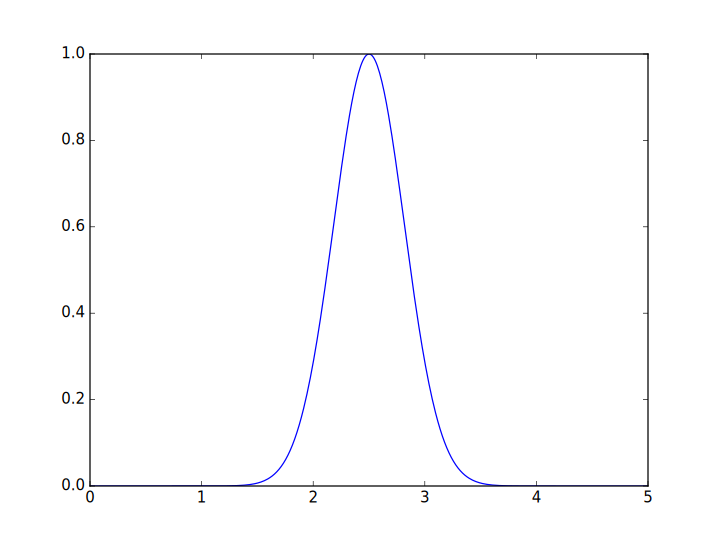
\includegraphics[width=0.5\textwidth,height=\textheight]{LocalizationFigures/singlehypothesis.*}
\caption{Single Hypothesis}
\end{figure}

\begin{figure}
\centering
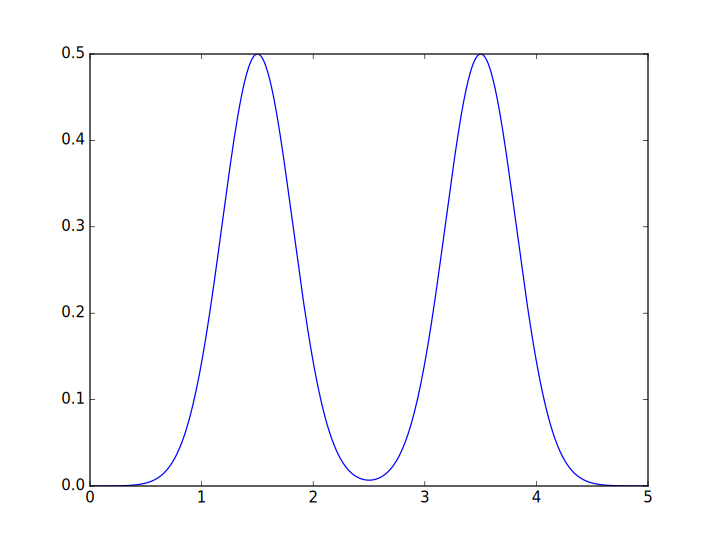
\includegraphics[width=0.5\textwidth,height=\textheight]{LocalizationFigures/multihypothesis.*}
\caption{Multihypothesis}
\end{figure}

Having multiple hypotheses seems a bit odd at first, but actually
arises. Imagine you have a Starbucks map - a map of a city that just
shows Starbucks. Also assume you drive up to a Starbucks. Now compare to
the map. You can now isolate your position to one of the \(n\) Starbucks
locations on the map. This is an example of multiple hypotheses. Only
until you receive additional information are you able to break the
ambiguity. With the reduced information available to a robot, this
situation arises when faced with vision system that use corners and
walls to generate landmarks.
